% \pagebreak[4]
% \hspace*{1cm}
% \pagebreak[4]
% \hspace*{1cm}
% \pagebreak[4]

\chapter{Mélange d'outils}

\graphicspath{ {Chapter2/Chapter2Figs/PNG/}
  {Chapter2/Chapter2Figs/PDF/} {Chapter2/Chapter2Figs/} }

Chaque dimension d'outil permet de déformer l'espace d'une autre
manière. Les points et courbes sont plus adaptés aux déformations
réalisées par rapport à un axe (rotation, torsion, fuselage). Les
surfaces et volumes sont, quant à eux, utilisés lors de déformations
plus générales.

Pourtant, sur le même ensemble de points, un utilisateur pourrait
souhaiter réaliser des déformations par rapport à un axe, mais aussi
plus générales. Aussi, les techniques les plus utilisées ces dernières
années, les \textit{cages de déformation} par exemple, définissent des
déformations \textit{globales}. Une déformation est dite globale
lorsque la modification d'un des sommets de contrôle de l'outil influe
sur l'ensemble des points de l'espace, même de façon
infinitésimale. Il est donc nécessaire de calculer des coordonnées
pour chaque point de l'espace par rapport à tous les sommets de
l'outil. De plus, pour réaliser des déformations sur des zones
précises, il faut que l'outil soit composé d'un grand nombre de
sommets, afin de diminuer l'influence des sommets les plus éloignés de
ces zones. On peut donc dire qu'il existe un lien entre la précision
d'une déformation et le nombre de sommets de l'outil associé. Or plus
il y a de sommets composant l'outil, plus le temps de calcul des
coordonnées sera important. Il n'est donc pas possible de réaliser des
déformations sur des zones très précises, sans avoir à calculer de
coordonnées pour tous les points de l'espace.

C'est sur cette problématique que les idées de mélange d'outils ont
été introduites.

\section{Etat de l'art}

On peut citer \cite{JBPS11} comme étant le premier a avoir proposé une
méthode permettant de mélanger plusieurs outils de déformation de
différentes dimensions.  C'est sur celui-ci que nous avons commencé à
travailler car la méthode nous semblait proche de ce que nous
souhaitions réaliser. Une lecture plus approfondie de l'article nous a
fait nous rendre compte que le fonctionnement n'était pas celui que
nous souhaitions. En effet, s'il semble s'appuyer sur des outils ayant
des dimensions différentes en fonction des zones à déformer, la
gestion interne repose uniquement sur des déformations d'outils de
dimension 0 (points). L'aspect "multidimensionnel" est donc uniquement
présent pour imposer des contraintes supplémentaires sur les calculs
de coordonnées. Par exemple pour des sommets reliés par une arête
l'article définit que les poids (permettant le calcul des coordonnées)
évoluent de façon linéaire le long de cette arête. De plus, cette
méthode passe par une minimisation de l'énergie laplacienne,
nécessitant une discrétisation de l'espace. Or c'est quelque chose que
nous souhaiterions éviter, à cause du temps de calcul requis par ces
opérations.
\\

\cite{GPCP13} quant à lui, propose une méthode permettant le mélange
d'outil de même dimension, en s'intéressant particulièrement aux cas
des surfaces, à travers les déformations à base de cage.  Nous nous
sommes intéressés à cet article de par sa récente publication (2013),
sa proximité avec \cite{Hur12}, un travail réalisé par un étudiant en
Master ISI en 2012, et de l'utilisation de cages de déformation, le
modèle semblant le plus pertinent parmi les outils de dimension 2.
L'idée est de réaliser un assemblage de différentes cages collées
ensembles le long de leurs arêtes et de considérer les coordonnées
d'un point de l'espace non seulement par rapport à sa cage
\textit{propre} (à comprendre la cage englobant le point de l'espace)
mais aussi par rapport aux cages adjacentes à celle-ci.

La méthode de cet article propose au premier abord une formulation
très claire. Celui-ci définit que la position d'un point de l'espace
n'est plus simplement constituée d'une combinaison linéaire des
positions des sommets de sa cage propre, mais résulte d'un mélange
entre les coordonnées calculées par rapport à la cage propre et aux
différentes cages \textit{jointure}. Une cage jointure correspond à
l'union des cages incidentes à un sommet de la cage propre. L'avantage
de ce genre de méthode est de localiser les déformations en les
limitant au voisinage de la cage incidente au sommet déplacé. On peut
donc avoir jusqu'à $n$ coordonnées différentes pour un même point de
l'espace, où $n$ correspond au nombre de sommets de la cage propre. Ce
qui au final fait perdre un des intérêts de la méthode, au moins en
partie, à savoir la réduction de la complexité en temps de calcul.

Cependant cette formulation claire cache d'autres formulations qui
semblent résulter d'un procédé empirique, dont le cheminement n'est
pas expliqué dans l'article. Ce qui rend la compréhension de l'utilité
de ces fonctions assez difficile.

\section{Cheminement de l'article}
Dans un premier temps, nous avons voulu reproduire le cheminement de
\cite{GPCP13}, pour comprendre quelles étaient les motivations
derrière l'existence de chaque fonction. Nous sommes donc partis de
l'expression globale de l'article, qui exprime la position d'un point
de l'espace comme étant une pondération des coordonnées de la cage
propre et de la cage jointure :
\begin{equation}
  p = (1 - \beta_i) T_i(p)  + \beta_i J_i(p) 
  \label{MELgen}
\end{equation}
Où $T_i(p)$ et $J_i(p)$ représentent les coordonnées du point p par
rapport à sa cage propre et sa cage jointure respectivement, et
$\beta_i$ représente la distance à l'arête $i$ de la cage propre. Pour
réduire la complexité du nombre de coordonnées qu'il sera nécessaire
de calculer, nous avons choisi de considérer une unique cage jointure
pour chaque point de l'espace, qui résulte de l'union de toutes les
cages incidentes aux sommets de l'arête considérée. Ainsi, pour chaque
point de l'espace le nombre de coordonnées à calculer sera de 2 au
maximum (une pour la cage propre, et une pour la cage jointure).

Le calcul de $\beta_i$ était proposé par l'article. Il s'agit de juger
la distance d'un point de l'espace par rapport à chaque arête
incidente à sa cage propre et à une autre cage. Pour cela, on utilise
les poids qui ont été utilisés lors du calcul de coordonnées par
rapport à la cage propre. La distance à une arête correspond donc à la
somme des poids associés à chaque sommet de l'arête :
\begin{equation}
  \beta_{i} = f(1 - \sum_{v \in E_i} \alpha_i)
\end{equation}
Où $E_i$ correspond à l'arête $i$ de la cage propre et $f(x)$
correspond à une fonction de lissage, permettant de faire varier la
taille de la zone d'infuence du mélange, tout en conservant un
estompement progressif :

\begin{equation}
  f(x) = \frac{1}{2} sin(\pi(\frac{x}{h}-\frac{1}{2}))
\end{equation}
Où $h$ représente la zone d'influence de l'arête, ce paramètre permet
de délimiter la zone où le mélange de coordonnées doit être fait
(figure \ref{MELpar}).

\begin{figure}[h]
  \begin{center}
    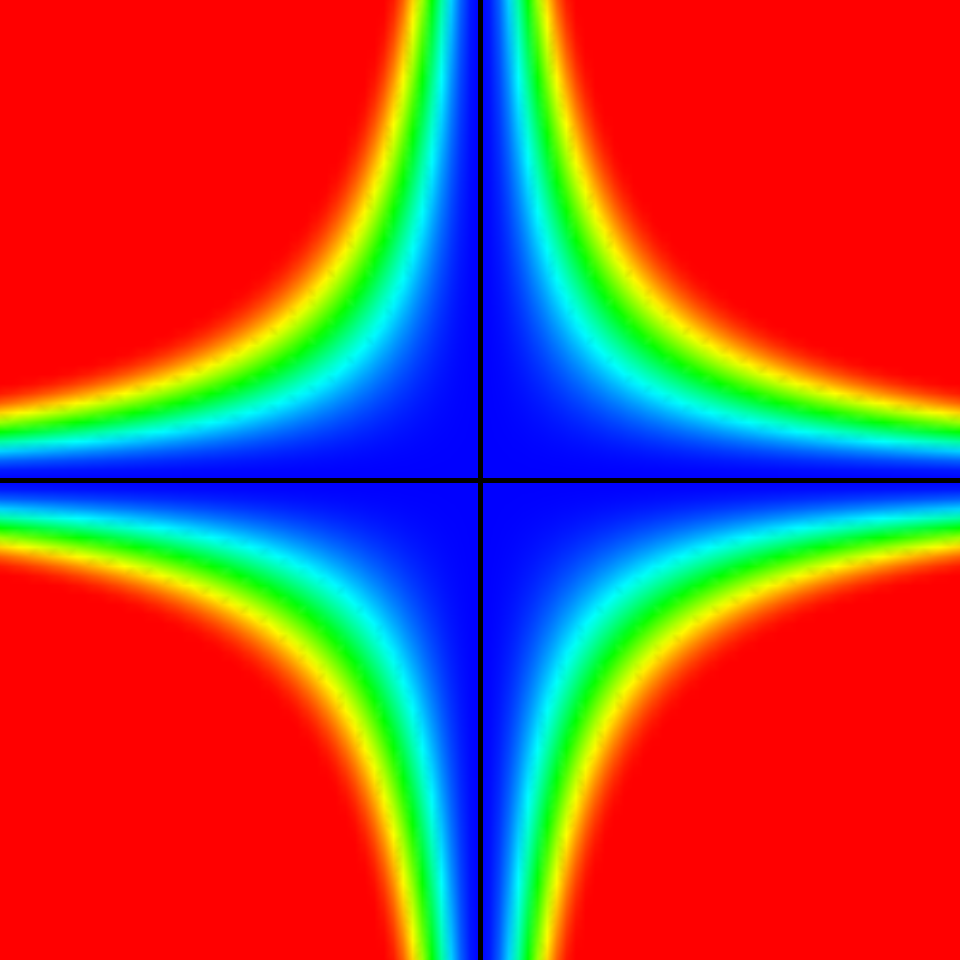
\includegraphics[scale=0.35]{starCage-0-2}
    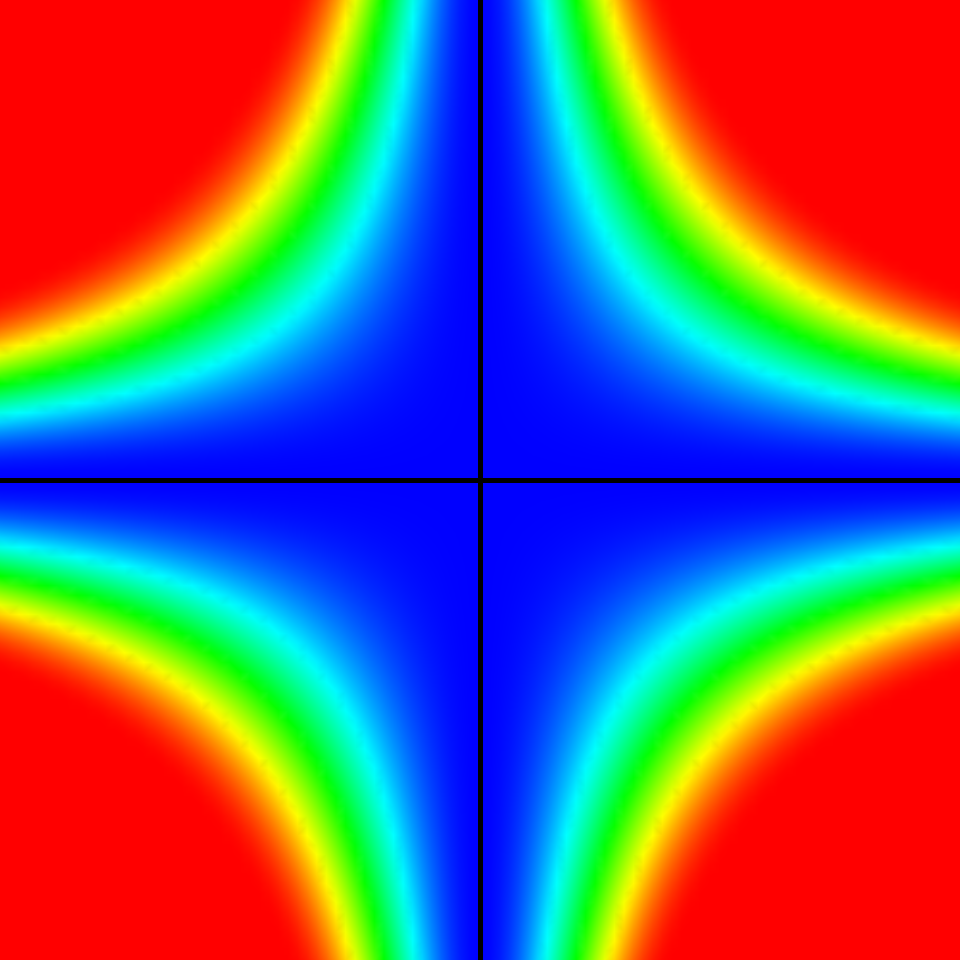
\includegraphics[scale=0.35]{starCage-0-4}
    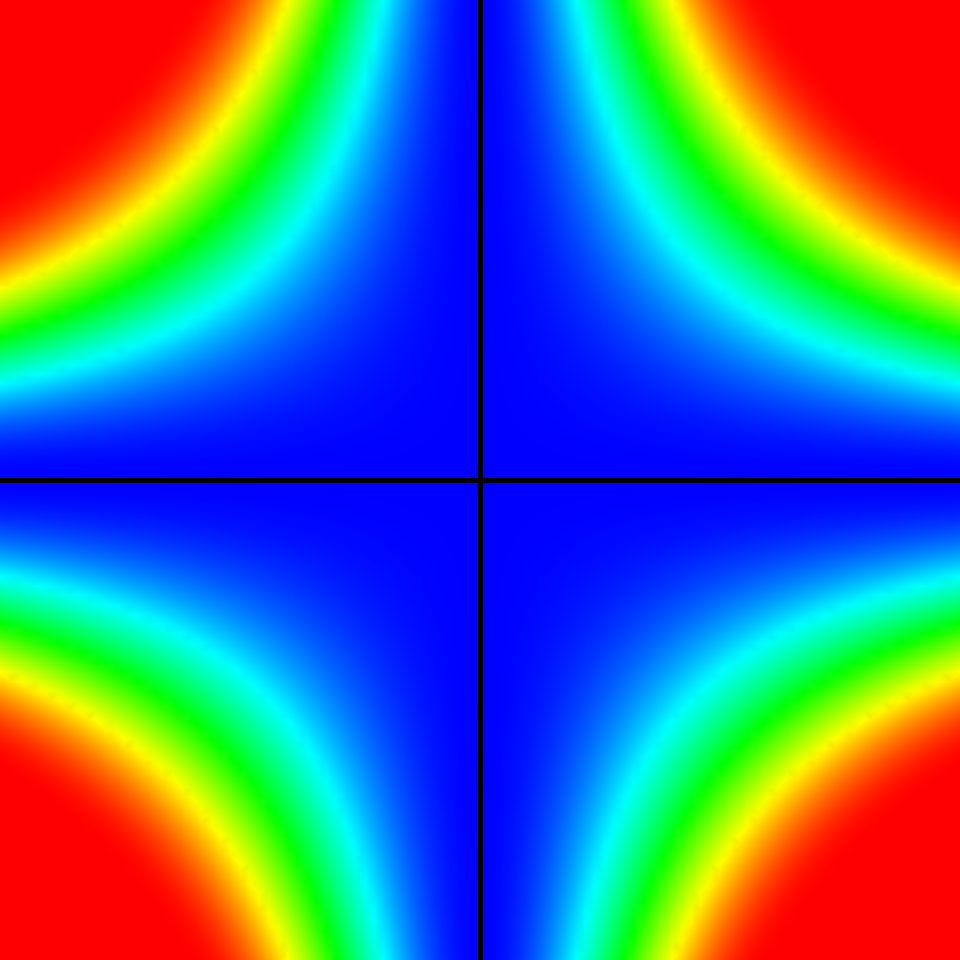
\includegraphics[scale=0.35]{starCage-0-6}
    \caption{Fonction de bordure calculée pour 4 cages (arêtes
      noires). Les variations de couleur représentent les variations
      de valeur de $\beta_i$ (la couleur bleu marine représentant une
      valeur de 1 et la couleur rouge une valeur de 0). En bleu les
      zones dites "de bordure" (i.e. points de l'espace proches d'une
      arête incidente à une autre cage). Valeurs de h : 0.2, 0.4 et
      0.6 pour les images à gauche, au centre et à droite
      respectivement.}
    \label{MELpar}
  \end{center}
\end{figure}

Comme $0 \leq \beta_i \leq 1$, on peut considérer $\beta_i$ comme le
pourcentage d'utilisation des coordonnées calculées par rapport à la
cage propre et par rapport à la cage jointure. D'après l'équation
\ref{MELgen}, lorsque $\beta_i$ vaut 1 (i.e. $p$ se trouve sur une
arête de la cage), la position de $p$ dépend uniquement de la
coordonnée calculée par rapport à la cage jointure $J_i$.

C'est là qu'apparaît le premier problème : Considérons une grille
constituée de 4 faces, chaque face constituant une cage. Toutes les
cages sont incidentes à un même sommet $s$. De ce fait, la zone autour
des arêtes incidentes à ce sommet sera fortement influencée par la
cage jointure composée de l'union des 4 cages. Afin que la cage
jointure reste un polygone, $s$ ne doit pas être considéré comme un
sommet de la cage jointure, car il fait partie de l'intérieur de
celle-ci. L'équation \ref{MELgen} nous indique que les zones les plus
proches des arêtes (i.e. là ou la valeur de $\beta_i$ vaut 1), ne sont
influencées que par la cage jointure. Et que, par conséquent, $s$ n'a
aucune influence sur ces points. On peut voir sur la figure
\ref{MELjoi} que les points les plus proches de $s$ sont en bleu, ce
qui signifie que $s$ n'a aucune influence (ou une influence très
minime) sur les points les plus proches, et une plus grande influence
sur les points plus éloignés. Ce qui est un comportement complètement
contre-intuitif et la déformation engendrée n'est pas du tout celle
attendue.

\begin{figure}[h]
  \begin{center}
    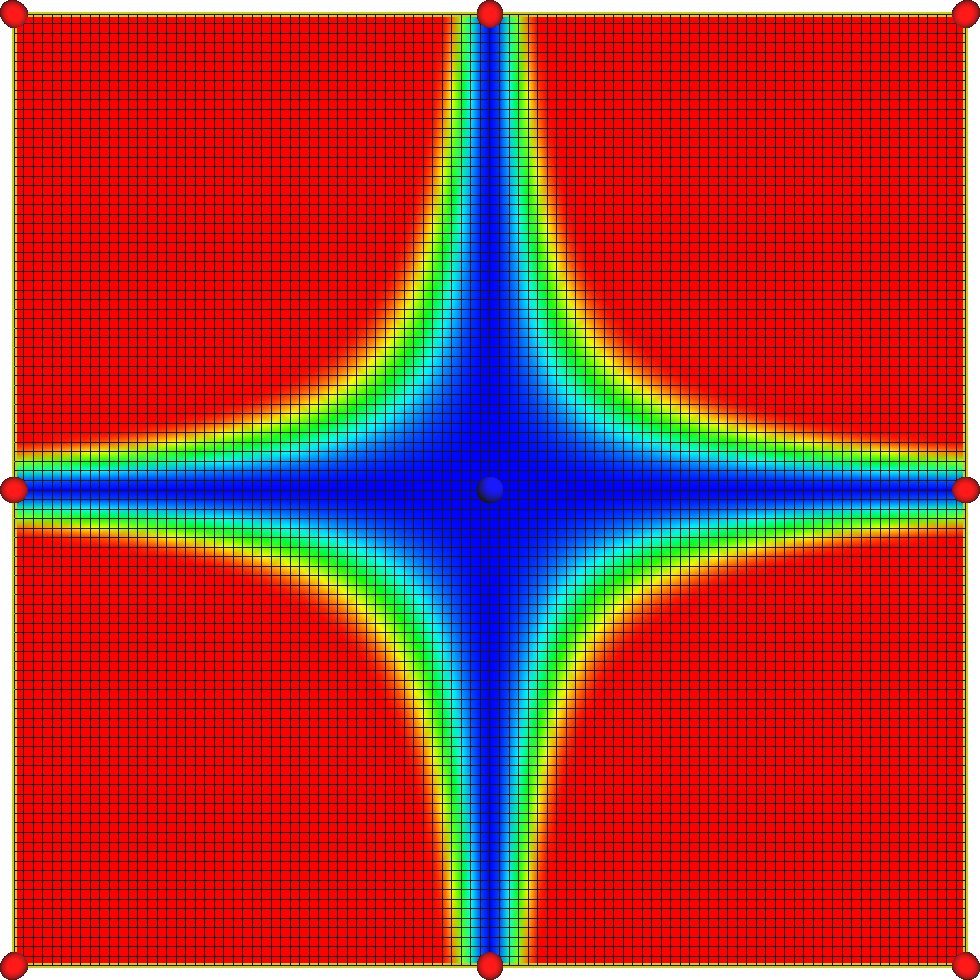
\includegraphics[scale=0.35]{starCage-jointure}
    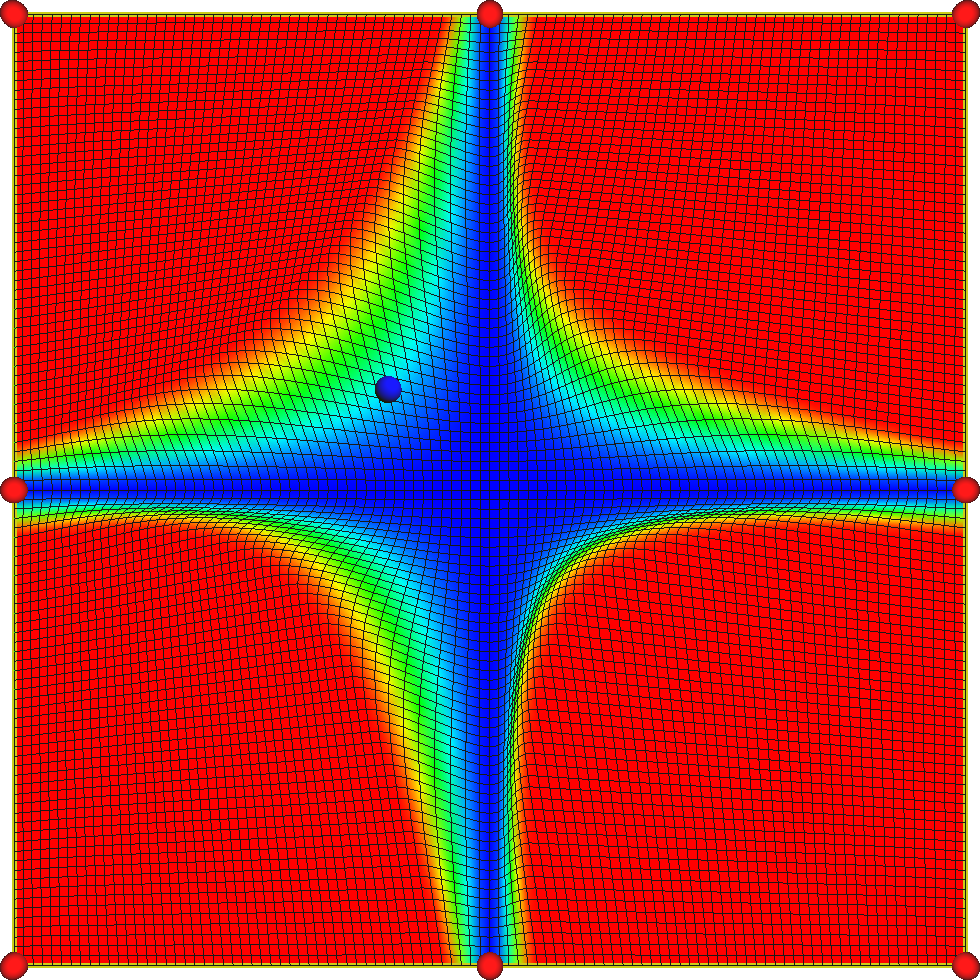
\includegraphics[scale=0.35]{starCage-jointure-deformation}
    \caption{Les boules rouges représentent les sommets de la cage
      jointure et la boule bleue représente le sommet $s$. Les zones
      en bleu ne sont pas modifiées par la translation de $s$}
    \label{MELjoi}
  \end{center}
\end{figure}

De la nous voyons la nécessité de rajouter un comportement spécifique
pour ces fameux sommets à l'intérieur de leur cage jointure. C'est une
des fonctions proposées par l'article. Ils résolvent ce problème au
travers de l'expression d'une déformation de type ponctuelle, associée
au sommet $s$. A partir de là, nous avons compris que la méthode
proposée \cite{GPCP13} n'était que le résultat d'une suite de
résolutions de cas spécifiques. Ce qui ne nous intéressait pas
vraiment, car un de nos critères principaux était l'utilisation d'une
formulation simple permettant d'exprimer les coordonnées de chaque
point de façon claire. De plus, cette méthode semblait difficilement
associable avec une méthode multidimensionnelle, car elle se basait
sur une fusion d'outils, ce qui semble difficilement réalisable entre
des outils de différentes dimensions.

Nous pouvons néanmoins relever l'avancée qu'apporte cet article dans
le domaine des déformations à base de cages. En effet, grâce au
mélange des diverses cages, la technique a permis de localiser la
déformation, tout en limitant le nombre de coordonnées à calculer pour
chaque point de l'espace. De plus, la possibilité d'utiliser
conjointement plusieurs systèmes de coordonnées différents permet de
choisir le plus adapté aux différentes déformations à effectuer.

C'est pour ça que la prochaine méthode s'inspire de cet article, en
ayant en tête cette idée de localisation de la déformation et de
limitation du temps de calcul des coordonnées.

\section{Méthode élaborée}
L'idée est de considérer des coordonnées \textit{étendues} pour chaque
cage, au lieu de considérer des unions de cages, et de réaliser un
mélange de coordonnées pour les points de l'espace qui sont sous
l'influence de plusieurs cages. On se base ici sur le fait que les
coordonnées barycentriques sont aussi définies à l'extérieur du
polygone de contrôle.

Pour vérifier la possibilité de réalisation d'une telle méthode, nous
avons commencé par travailler sur un exemple simple, le cage d'une
cage unique déformant des points de l'espace à la fois à l'intérieur
et à l'extérieur. Il s'agissait de voir le comportement de la
déformation, afin de savoir s'il était possible de considérer des
coordonnées à la fois à l'intérieur et à l'extérieur. Car dans la
littérature, les coordonnées n'ont été utilisées que pour déformer des
points à l'intérieur du polygone et jusqu'à son bord.


% ------------------------------------------------------------------------


%%% Local Variables: 
%%% mode: latex
%%% TeX-master: "../thesis"
%%% End: 
